%% ------------------------------------------------------------------------- %%
\chapter{Fundamentação Teórica}
\label{cap:fundamentacao-teorica}

O problema de remoção de ruído telúrico em sinais astronômicos é de natureza interdisciplinar, o que implica na necessidade de compreender tanto a teoria da astronomia sobre espectros estelares, quanto a teoria da computação sobre processamento de sinais digitais.
Neste capítulo são descritos conceitos básicos em espectroscopia astronômica e processamento de sinais digitais que caracterizam o problema da contaminação telúrica de espectros estelares.

\section{Espectroscopia Astronômica}

A espectroscopia é a técnica de dividir a luz, ou mais precisamente, a radiação eletromagnética, proveniente de um objeto em seus comprimentos de onda constituintes, o que resulta na formação de um espectro. Quando aplicada na astronomia, tem como objeto de estudo o espectro de radiação eletromagnética de diversos corpos celestes, como estrelas, planetas, nebulosas, galáxias e núcleos galácticos ativos.

Diferentes tipos de objetos celestes produzem diferentes tipos de espectro:  contínuo, de absorção e de emissão. Um espectro contínuo é um vetor de todos os comprimentos de ondas do espectro eletromagnético, arranjado de forma contínua. Ele é gerado pela observação de um corpo opaco quente, que seria o equivalente a observar diretamente o núcleo de uma estrela sem intervenção de matéria. Um espectro de absorção, ou espectro de linhas escuras, é gerado por um gás transparente frio em frente ao corpo opaco quente e está associado à absorção dos fótons da radiação em determinados comprimentos de onda. E por último, o espectro de emissão, ou espectro de linhas brilhantes, é gerado por um gás transparente que foi excitado por uma fonte de energia próxima, o que resulta na emissão de fótons de comprimentos de onda específicos. 

\begin{figure}[htb]
\centering
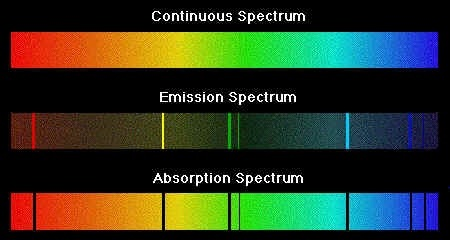
\includegraphics[width=10cm]{figuras/spectypes.jpg}
\caption{Os três tipos de espectro}
\label{fig:spectrum-types}
\end{figure}

Um objeto astronômico que é muito estudado pelos seus espectros são as estrelas. Por serem objetos quentes, rodeados de gases mais frios, estrelas emitem um espectro contínuo com linhas de absorção em comprimentos de onda característicos.

No final do século XIX, astrônomos perceberam que a análise cuidadosa do espectro de uma estrela fornece uma riqueza de detalhes sobre ela, incluindo temperatura efetiva, velocidade de rotação, velocidade de translação, densidade, composição química e metalicidade. Com a observação rotineira de espectros estelares em grandes números, estes pesquisadores notaram que era possível agrupar as estrelas baseado em suas características espectrais e assim surgiram diversos sistemas de classificação estelar. 

O sistema moderno de classificação de estrelas foi adotado em 1910 e foi criado por um time do observatório da Universidade de Harvard. Este sistema baseia-se nas intensidades relativas das linhas de absorção presentes no espectro. As variações nas linhas espectrais para diferentes estrelas são devidas principalmente à diferença de temperatura das camadas externas de gás na estrela, logo o sistema de classificação espectral é baseado na temperatura efetiva da estrela. 

As classes espectrais do sistema, em ordem decrescente de temperatura efetiva da estrela são: O, B, A, F, G, K, M. Cada uma dessas classes se subdivide em 10 (com os números de 0 a 9), sendo 0 a mais quente dentro da classe e 9 a mais fria.

\begin{figure}[htb]
\centering
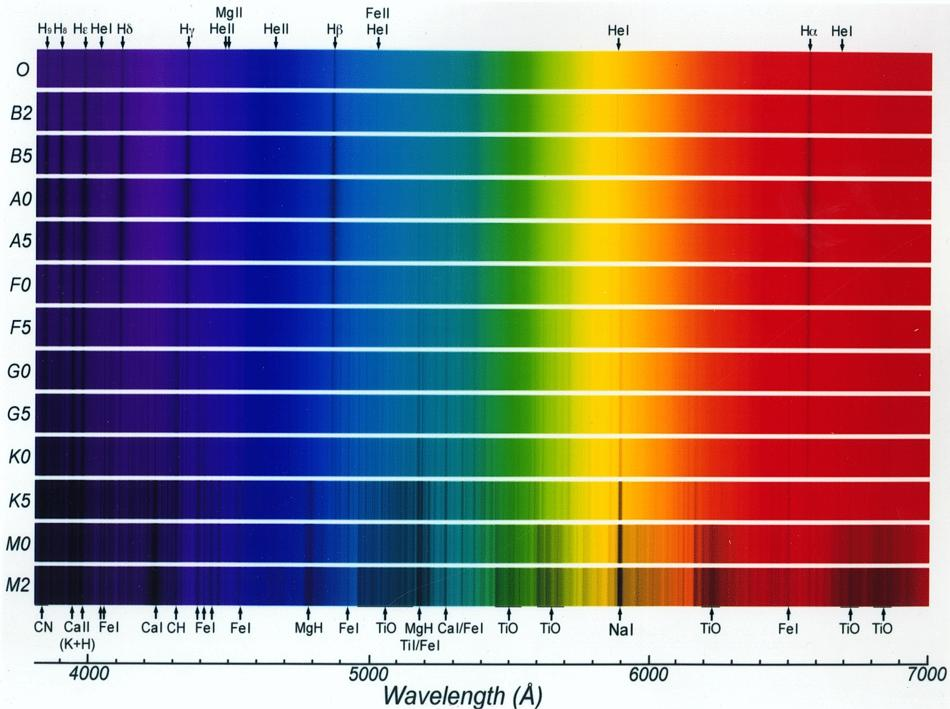
\includegraphics[width=10cm]{figuras/Spectra_Briley.jpg}
\caption{Tipos de espectro estelar}
\label{fig:stellar-spectrum-types}
\end{figure}

Na figura ~\ref{fig:stellar-spectrum-types}, é possível observar como diferentes linhas de absorção e bandas moleculares variam em força conforme a temperatura efetiva, ou tipo espectral, da estrela muda.

Os tipos espectrais das estrelas continuam sendo uma parte essencial para a pesquisa em astronomia, seja para auxiliar na descoberta de exoplanetas ou na interpretação da história da evolução das galáxias. 

\section{Contaminação Telúrica}

Para realizar as pesquisas que necessitam de espectros estelares, é necessário capturá-los com os instrumentos corretos. O instrumento que divide a radiação eletromagnética de objetos celestes em seus respectivos comprimentos de onda é o espectrógrafo, que pode estar presente tanto em telescópios terrestres quanto telescópios espaciais.

A maioria das observações astronômicas são feitas em telescópios terrestres, ou seja, a partir do solo, e nesse caso, nem toda luz irradiada por um objeto celestre consegue ser capturada pelo espectrógrafo. Isto acontece pois, ao atravessar a atmosfera terrestre o sinal astronômico interage com moléculas como vapor de água e oxigênio o que resulta na formação de novas linhas no espectro observado. Estas linhas são chamadas de linhas telúricas.

As linhas telúricas, quando misturadas no espectro original, contribuem para a criação de uma observação distorcida ou contaminada. A menos que seja corrigida, esta contaminação pode produzir erros e introduzir ruídos que reduzem a precisão dos dados observados, e consequentemente, dificultam o avanço de diversas pesquisas astronômicas.

Existem alguns procedimentos típicos usados hoje em dia para remover as linhas telúricas de um espectro observado, também chamado de espectro de ciência. Um método popular consiste em aplicar uma divisão simples entre o espectro da observação e uma referência telúrica. Esta referência telúrica pode ser obtida de duas maneiras: através de um catálogo de estrelas padrão ou da simulação de um espectro atmosférico teórico.

As estrelas padrão são estrelas quentes em rotação rápida e de tipo espectral B ou A. Elas são escolhidas pois seus espectros não possuem características marcantes além de fortes linhas de hidrogênio. Para que o espectro de uma estrela padrão seja usado como uma referência telúrica, é necessário observá-la próxima em tempo, posição no céu e condições atmosféricas do espectro de ciência. Contudo, existem várias limitações fundamentais no nível de correção que pode ser obtido com o método da estrela padrão. Primeiramente, características estelares ainda podem estar presentes no espectro da estrela padrão, evidenciando que ela não é um modelo preciso da transmissão radiativa da atmosfera. Além disso, o tempo e a direção de observação das duas estrelas não é exatamente o mesmo, o que significa que a assinatura atmosférica de ambos os espectros também será diferente.

Devido às limitações listadas das estrelas padrão, foi criado um método mais sofisticado e automatizado para obter uma referência telúrica: softwares de simulação do espectro atmosférico. Estes softwares utilizam modelos de transmissão radiativa da atmosfera para criar um espectro telúrico sintético, cujas condições de simulação são muito próximas às condições de observação da estrela de ciência. O modelo de transmissão atmosférica mais utilizado hoje em dia é o \textit{Line-By-Line Radiative Transfer Model (LBLRTM)}, que fornece cálculos de radiância espectral com precisão e eficiência. (seifhart e hitran, molecfit)   


\section{Sinal espectral}
\begin{itemize}
    \item O que é um sinal digital e como ele está sendo usado nesse caso (espectro estelar)
    \item Como o sinal é criado (CCD e redução de dados)
    \item filtros e pré-processamento de sinais
    \item operações no sinal todo (como estamos considerando o problema)
\end{itemize}


